\section{Implementation and results}\label{sec:results}
\subsection{Task 1: Model development}
\begin{figure}[ht]
    \begin{subfigure}{.5\textwidth}
        \centering
        % include first image
        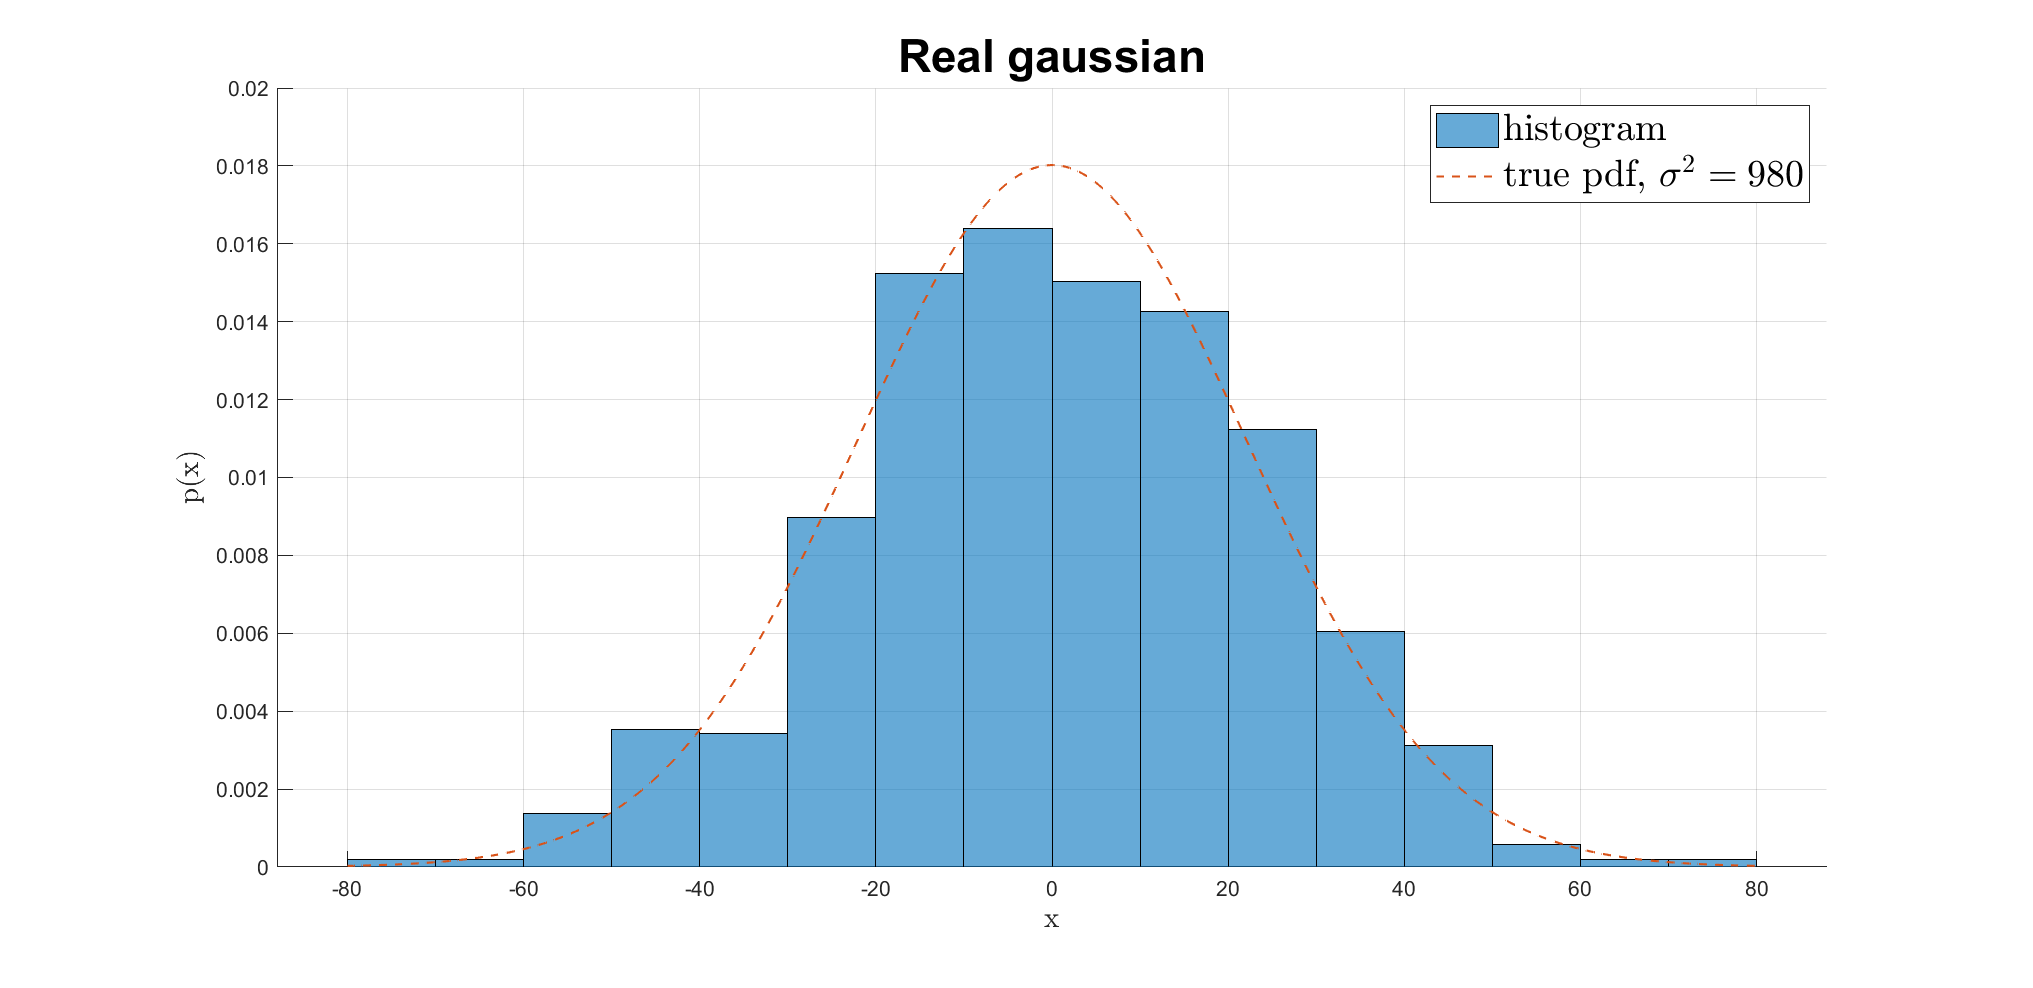
\includegraphics[width=.8\linewidth]{figures/re_gauss.eps}  
        \caption{The histogram of Re(S(k))$~$Gaussian}
        \label{fig:re_gauss}
    \end{subfigure}
    \begin{subfigure}{.5\textwidth}
        \centering
        % include second image
        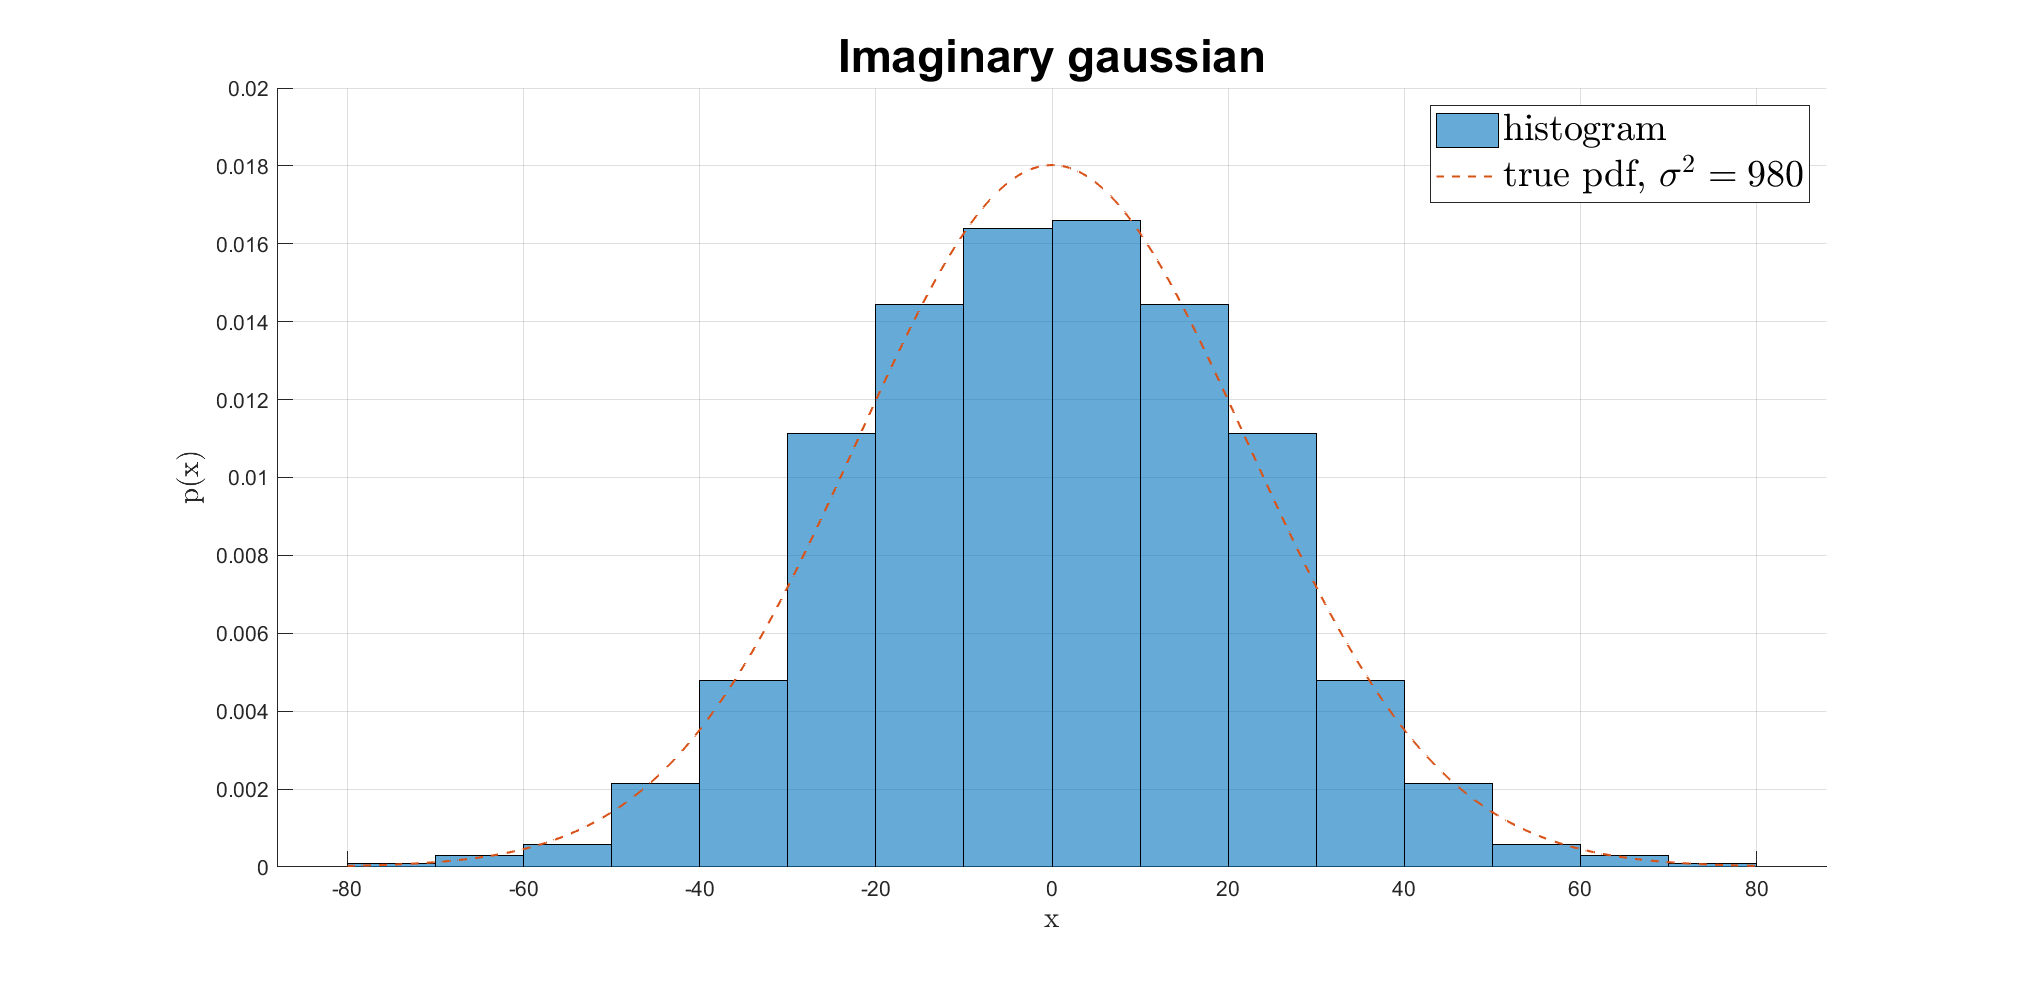
\includegraphics[width=.8\linewidth]{figures/im_gauss.eps}  
        \caption{The histogram of Im(S(k))$~$Gaussian}
        \label{fig:im_gauss}
    \end{subfigure}
    \begin{subfigure}{.5\textwidth}
        \centering
        % include third image
        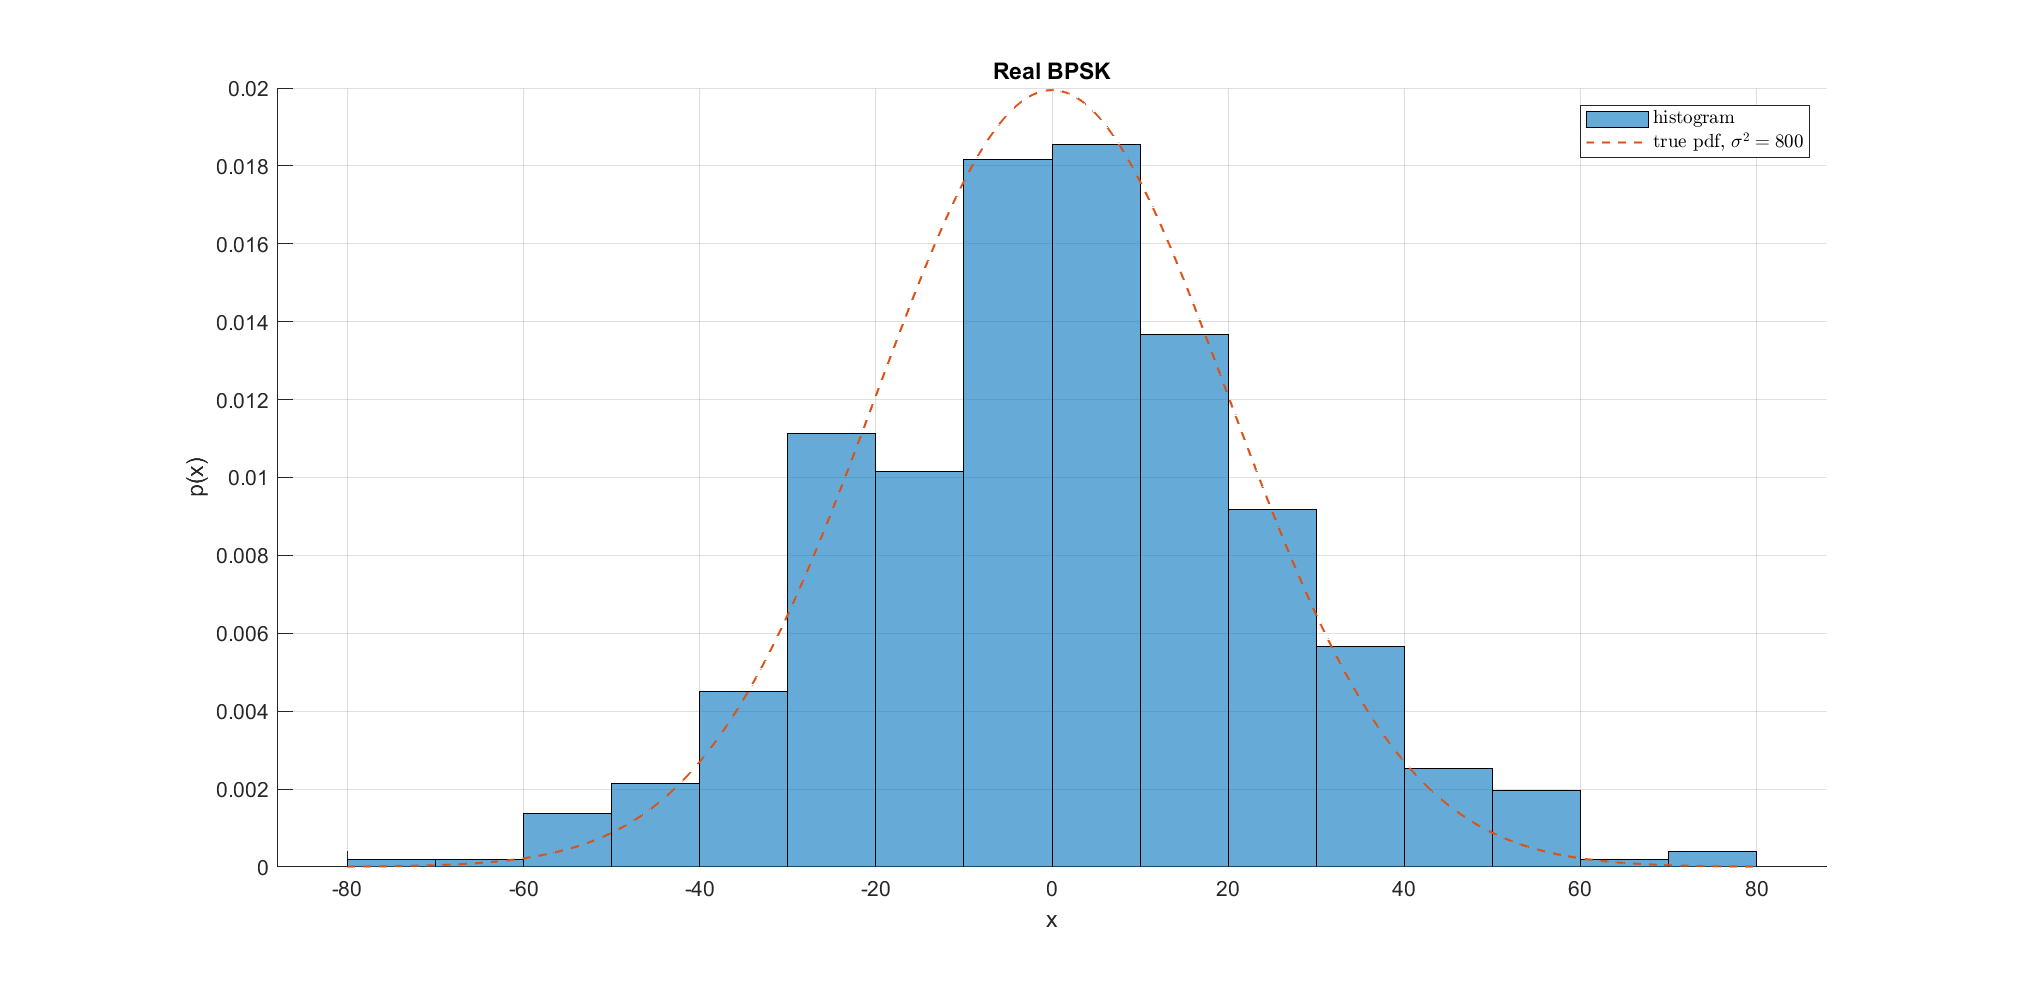
\includegraphics[width=.8\linewidth]{figures/re_bpsk.eps}
        \caption{The histogram of Re(S(k))$~$BPSK}
        \label{fig:re_bpsk}
    \end{subfigure}
    \begin{subfigure}{.5\textwidth}
        \centering
        % include fourth image
        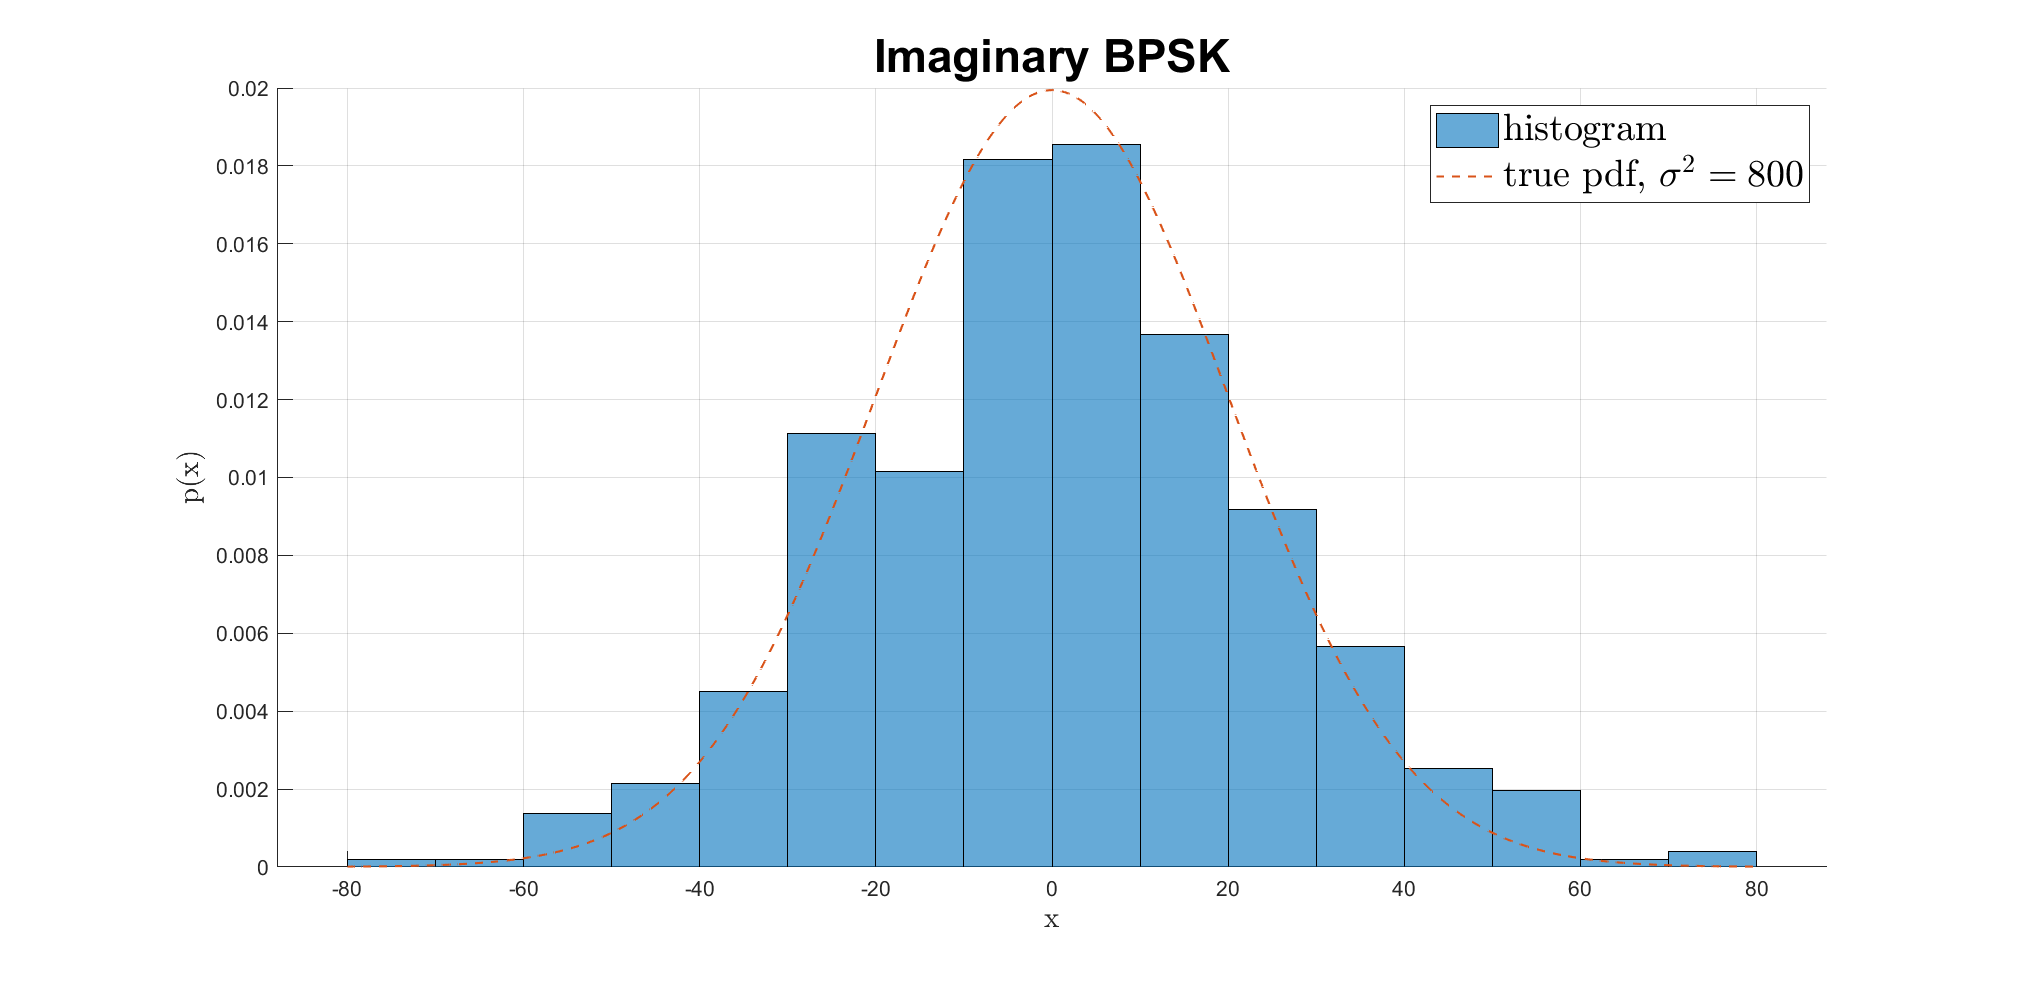
\includegraphics[width=.8\linewidth]{figures/im_bpsk.eps}
        \caption{The histogram of Im(S(k))$~$BPSK}
        \label{fig:im_bpsk}
    \end{subfigure}
    \caption{The histograms compared to pdf of gaussian}
    \label{fig:gauss}
\end{figure}

\subsection{Task 2: One-sample-detector}
In this task only one sample is used meaning that the detection problem is in this case:
\begin{align}
    H_0 &: x(0) = w(0)\nonumber\\
    H_1 &: x(0) = s(0)+w(0)\nonumber
\end{align}
It is given from the problem that $w\thicksim\mathbb{C}\mathcal{N}(0, \sigma_w^2)$ and $s\thicksim\mathbb{C}\mathcal{N}(\mu_s, \sigma_s^2)$ which means that under $H_0$, $x$ is from same distribution as $w$ and thus a complex gaussian with same mean and variance as $w$. Under $H_1$, which is a sum of two complex gaussian distribution, $x$ also is from a complex gaussian distribution, however the mean and variance needs to be calculated.
The mean of $x(0)$ under $H_1$ is\todo{Usikker på om det er vits med disse utregningene}
\begin{align}
    \mathbb{E}\{x(0)\} & = \mathbb{E}\{s(0)+w(0)\}\nonumber\\
    & = \mathbb{E}\{s(0)\} + \mathbb{E}\{w(0)\}\nonumber\\
    & = \mu_s + 0 = \mu_s\nonumber
\end{align} 
The variance of $x(0)$ under $H_1$ is
\begin{align}
    \mathrm{Var}\{x(0)\} & = \mathrm{Var}\{s(0)+w(0)\}\nonumber\\
    & = \mathrm{Var}\{s(0)\} + \mathrm{Var}\{w(0)\}\nonumber\\
    & = \sigma_s^2+\sigma_w^2\nonumber
\end{align}
Meaning that
\begin{align}
    p(x;H_0) & = p_0(x) = \frac{1}{\sigma_w^2\pi}e^{-\frac{|x|^2}{\sigma_w^2}}\\
    p(x;H_1) & = p_1(x) = \frac{1}{(\sigma_w^2+\sigma_s^2)\pi}e^{-\frac{|x-\mu_s|^2}{\sigma_s^2+\sigma_w^2}}
\end{align}
Setting up the LRT:
\begin{align}
    L(x) & = \frac{p_1(x(0))}{p_0(x(0))} = \frac{\frac{1}{(\sigma_w^2+\sigma_s^2)\pi}e^{-\frac{|x(0)-\mu_s|^2}{\sigma_s^2+\sigma_w^2}}}{\frac{1}{\sigma_w^2\pi}e^{-\frac{|x(0)|^2}{\sigma_w^2}}}\nonumber\\
    & = \frac{\sigma_w^2}{\sigma_w^2+\sigma_s^2}e^{-\frac{1}{\sigma_w^2+\sigma_s^2}|x(0)-\mu_s|^2+\frac{1}{\sigma_w^2}|x(0)|^2}\nonumber
\end{align}
Since it was shown in task 1 that $\mu_s \simeq 0$ this can be used to simplify the caluclations. The decision rule is to choose $H_1$ when $L(x) \geq \lambda$, since $L(x(0))$ is a monotonically increasing function then the inequality holds for $\ln L(x(0)) \geq \ln\lambda$.
\begin{align}
    \ln L(x(0)) = \ln (\sigma_w^2)-\ln (\sigma_w^2+\sigma_s^2)-\frac{1}{\sigma_w^2+\sigma_s^2}|x(0)|^2+\frac{1}{\sigma_w^2}|x(0)|^2 \geq \ln\lambda\nonumber\\
    (\frac{1}{\sigma_w^2}+\frac{1}{\sigma_s^2+\sigma_w^2})|x(0)|^2 \geq \ln\lambda-\ln (\frac{\sigma_w^2}{\sigma_w^2+\sigma_s^2})\nonumber\\
    |x(0)|^2 = x_R(0)^2+x_I(0)^2 \geq \frac{\sigma_w^2(\sigma_w^2+\sigma_s^2)}{\sigma_s^2}(\ln\lambda-\ln (\frac{\sigma_w^2}{\sigma_w^2+\sigma_s^2})) = \lambda'\nonumber
\end{align}
This also means that the decision rule is to choose $H_1$ when $|x(0)|^2\geq\lambda'$ and choose $H_0$ when $|x(0)|^2<\lambda'$ where
\begin{equation}
    \lambda' = \frac{\sigma_w^2(\sigma_w^2+\sigma_s^2)}{\sigma_s^2}(\ln\lambda-\ln (\frac{\sigma_w^2}{\sigma_w^2+\sigma_s^2}))
\end{equation}\label{eq:lambda_prime}
\subsection{Task 3: Performance of the one-sample detector}
\begin{figure}[ht]
    \begin{subfigure}{.5\textwidth}
        \centering
        % include first image
        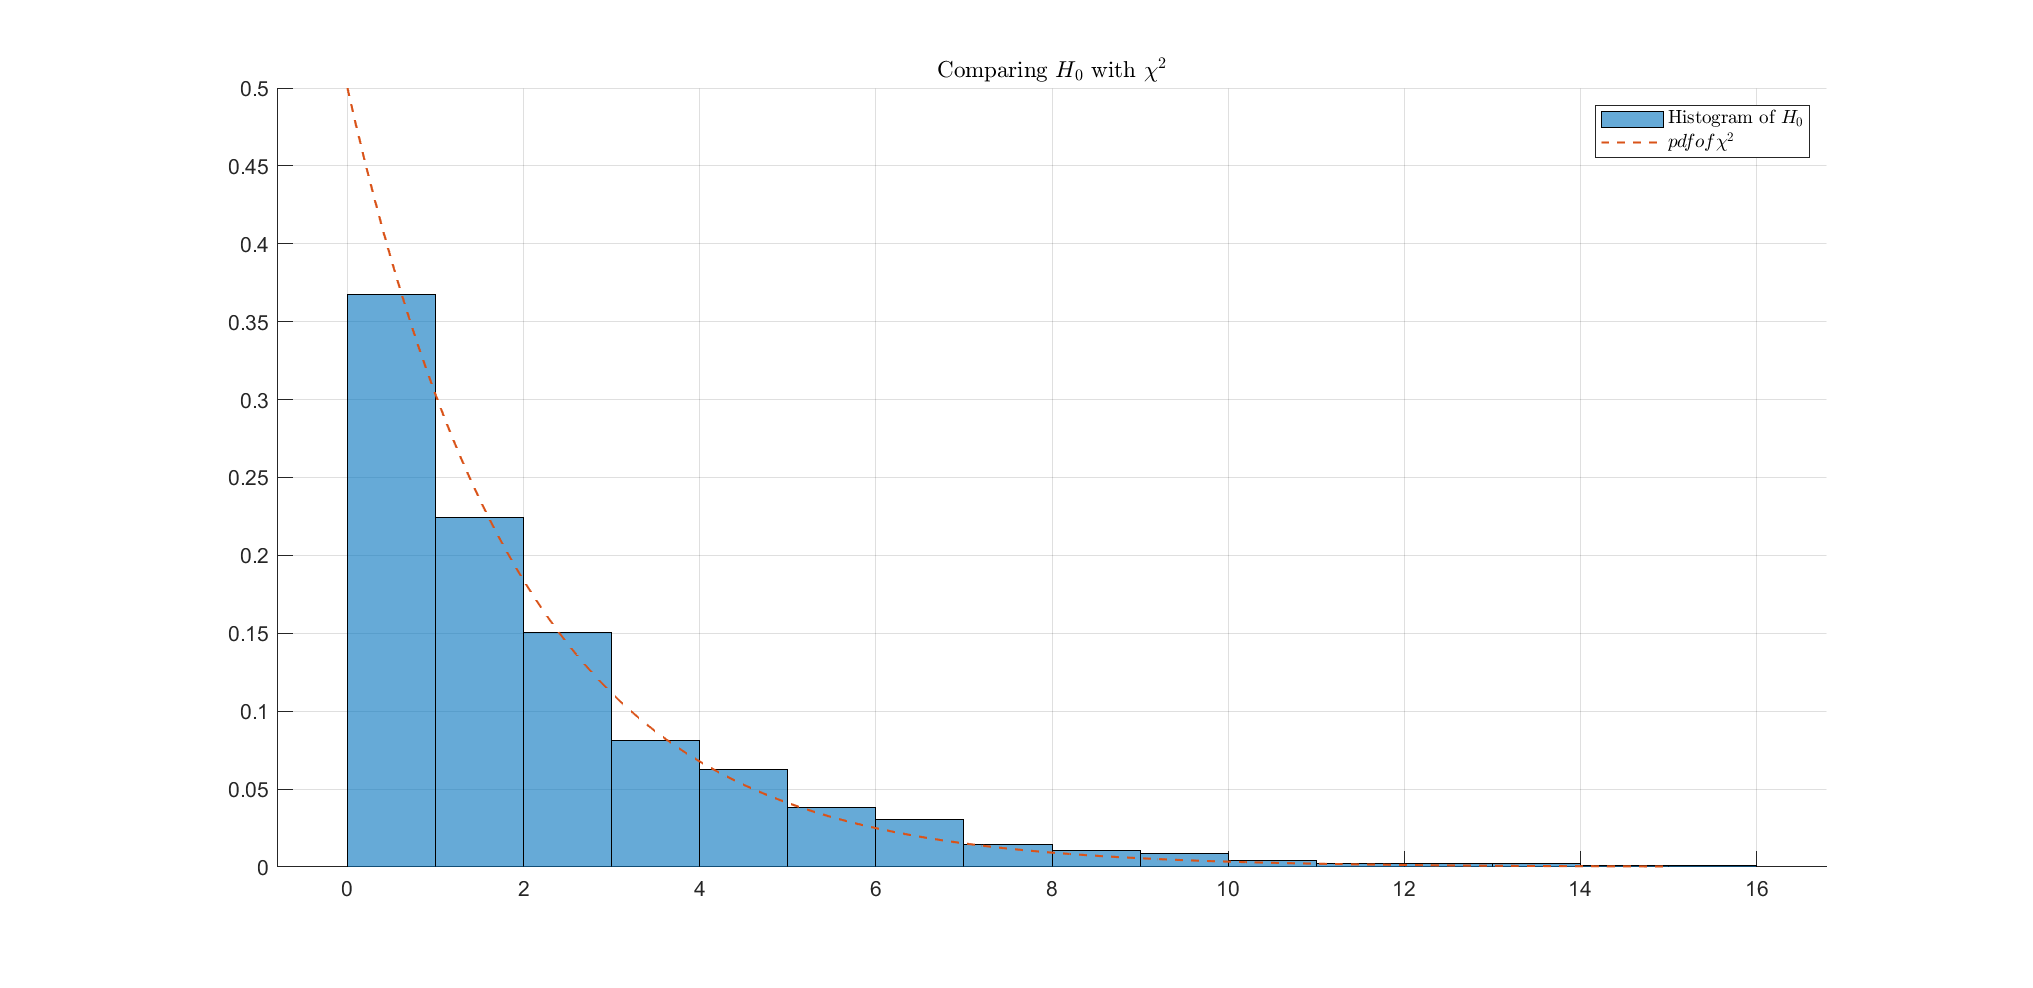
\includegraphics[width=.8\linewidth]{figures/chi_square_h0.eps}  
        \caption{The histogram of \eqref{eq:chi_sq_h0}}
        \label{fig:chi_sq_h0}
    \end{subfigure}
    \begin{subfigure}{.5\textwidth}
        \centering
        % include second image
        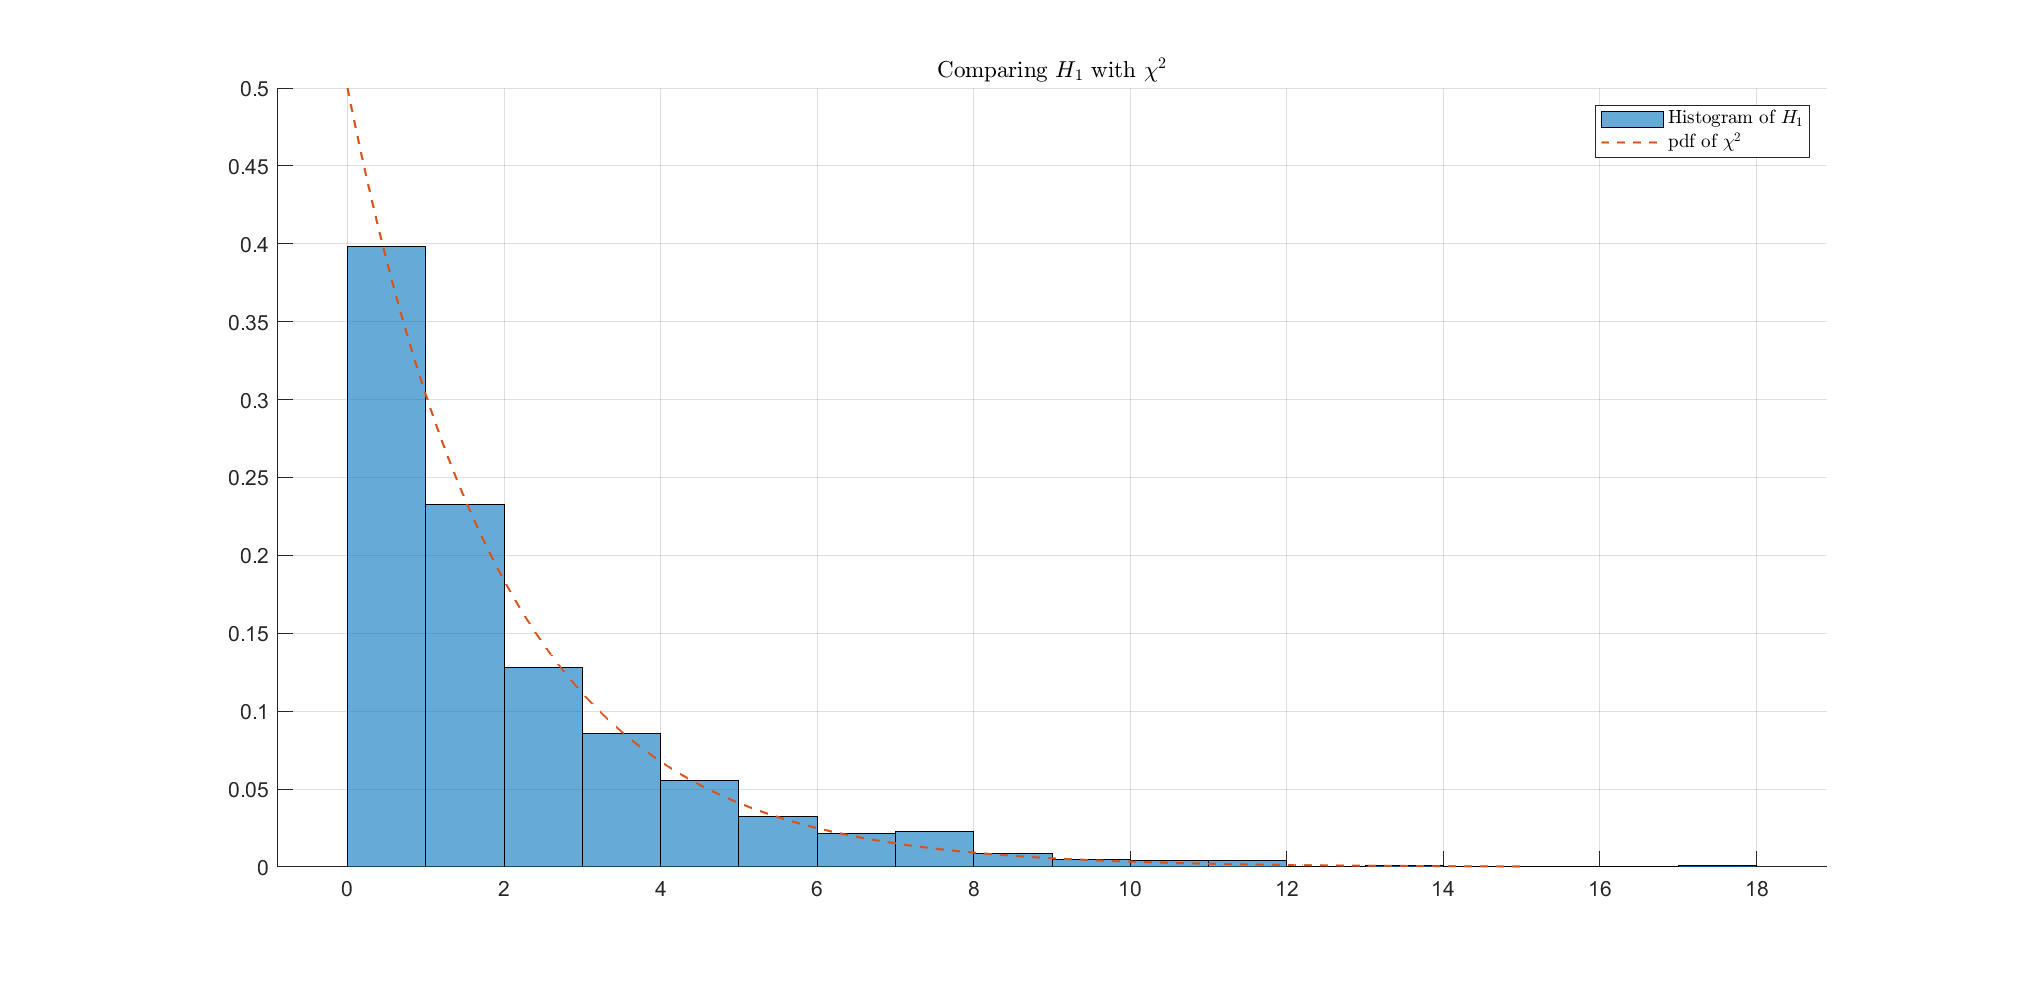
\includegraphics[width=.8\linewidth]{figures/chi_square_h1.eps}  
        \caption{The histogram of \eqref{eq:chi_sq_h1}}
        \label{fig:chi_sq_h1}
    \end{subfigure}
\end{figure}
The probability for false alarm is the probability that $|x(0)|^2>\lambda'$, assumed that it is actually the null hypothesis that is correct. Instead of using the complex gaussian pdf we have shown that $2\frac{|x(0)|^2}{\sigma^2}$ under $H_0$ and $H_1$ can be approximated to be $\chi^2$ distributed meaning that
\begin{align}
    P_{FA} & = \text{Prob}\{|x(0)|\geq\lambda'\vert H_0\}\nonumber\\
    & = \frac{\sigma_w^2}{2}\int_{\lambda'}^{\infty}\frac{e^{-\frac{x}{2}}}{2}dx\nonumber\\
    & = -\frac{\sigma_w^2}{2}e^{-\frac{x}{2}}\bigg\rvert_{\lambda'}^{\infty}\nonumber\\
    & = \frac{\sigma_w^2}{2}e^{-\frac{\lambda'}{2}}\nonumber
\end{align}
Which only holds when $\lambda'>0$.\\
Furthermore the probability for detection is
\begin{align}
    P_D & = \text{Prob}\{|x(0)|\geq\lambda'\vert H_1\}\nonumber\\
    & = \frac{\sigma_w^2+\sigma_s^2}{2}\int_{\lambda'}^{\infty}\frac{e^{-\frac{x}{2}}}{2}dx\nonumber\\
    & = -\frac{\sigma_w^2+\sigma_s^2}{2}e^{-\frac{x}{2}}\bigg\rvert_{\lambda'}^{\infty}\nonumber\\
    & = \frac{\sigma_w^2+\sigma_s^2}{2}e^{-\frac{\lambda'}{2}}\nonumber
\end{align}
Which also only holds for $\lambda'>0$\\
\subsection{Task 4: Generalized for multiple samples}
We take the one-sample-detector a step further and generalize it to use it for multiple samples. That is that the likelihood function is used to calculate the LRT so that we get
\begin{align}
    \ln L(x) & = \ln\prod_{n=0}^{K-1}\frac{1}{(\sigma_w^2+\sigma_s^2)\pi}e^{-\frac{|x(n)|^2}{\sigma_s^2+\sigma_w^2}}-\ln\prod_{n=0}^{K-1}\frac{1}{\sigma_w^2\pi}e^{-\frac{|x(n)|^2}{\sigma_w^2}}\nonumber\\
    & = \sum_{n=0}^{K-1}\left(\ln\frac{\sigma_w^2}{\sigma_w^2+\sigma_s^2} + \frac{|x(n)|^2}{\sigma_w^2}-\frac{|x(n)|^2}{\sigma_w^2+\sigma_s^2} \right)\nonumber\\
    & = \sum_{n=0}^{K-1}\left(\ln\frac{\sigma_w^2}{\sigma_w^2+\sigma_s^2} + \frac{\sigma_s^2}{\sigma_w^2(\sigma_w^2+\sigma_s^2)}|x(n)|^2\right)\geq\ln\lambda\nonumber
\end{align}
So the decision rule ends up being to choose $H_1$ when
\begin{equation}
    \sum_{n=0}^{K-1}|x(n)|^2 \geq \frac{\sigma_w^2(\sigma_w^2+\sigma_s^2)}{\sigma_s^2}\left(\ln\lambda-K\ln\frac{\sigma_w^2}{\sigma_w^2+\sigma_s^2}\right) = \lambda'
\end{equation}
\begin{enumerate}[i]
    \item What is this chapter about
    \item Matlab implementation
    \item Any specific Matlab m-commands used?
    \item A flow-diagram is recommended
    \item Results (use figures/tables if possible)
    \item Discussion of results
    \item Matlab code (documented) in appendix
\end{enumerate}